
%(BEGIN_QUESTION)
% Copyright 2010, Tony R. Kuphaldt, released under the Creative Commons Attribution License (v 1.0)
% This means you may do almost anything with this work of mine, so long as you give me proper credit

Den roterende ekvivalenten til {\it kraft} er noe som kalles {\it dreiemoment}. Diagrammet under viser den fysiske definisjonen i en situasjon der et tau utøver kraft på omkretsen av en trinse:

$$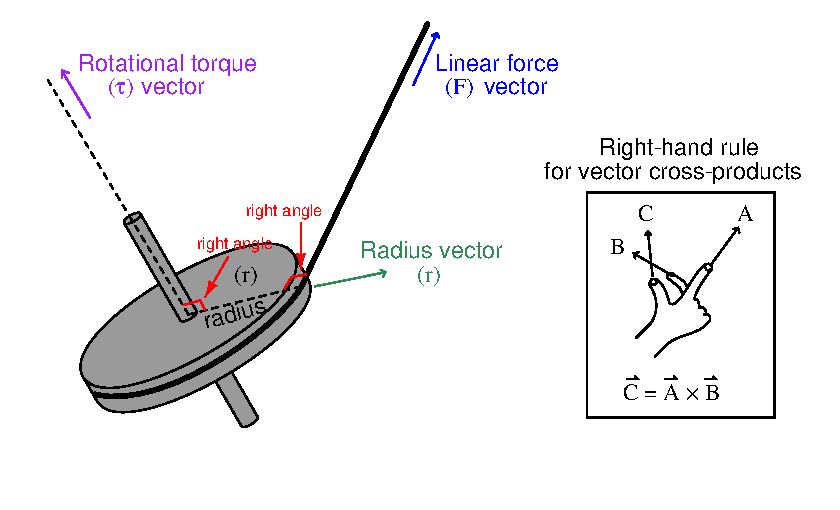
\includegraphics[width=15.5cm]{i01403x03.eps}$$

Matematisk er dreiemoment produktet av kraftvektoren og radiusvektoren vinkelrett på kraften (kalt ``momentarm''):

$$\vec \tau = \vec r \times \vec F$$

Basert på denne formelen: Bestem korrekt måleenhet for dreiemoment, gitt kraft i {\it pounds} og radius i {\it feet}.

\vskip 10pt

Deretter: Beregn hvor stort dreiemoment som påføres bolthodet av skiftenøkkelen, gitt at kraften er 82 ounces og momentarmens lengde er 17 inches:

$$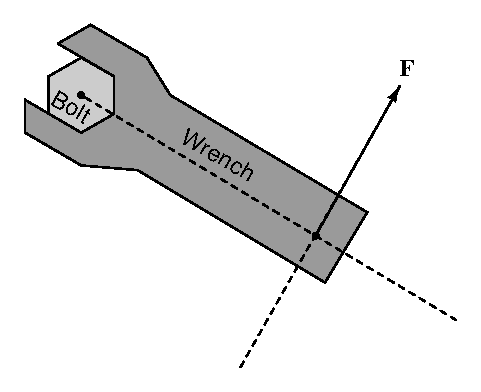
\includegraphics[width=15.5cm]{i01403x01.eps}$$

\filbreak

\vskip 20pt \vbox{\hrule \hbox{\strut \vrule{} {\bf Forslag til sokratisk diskusjon} \vrule} \hrule}

\begin{itemize}
\item{} En viktig detalj er at selv om formelen for å beregne dreiemoment innebærer multiplikasjon av {\it pounds} kraft og {\it feet} avstand, akkurat som formelen for arbeid ($W = Fx$), er dreiemoment i pound-feet definitivt ikke det samme som arbeid i foot-pounds. Gi et praktisk eksempel som viser hvordan dreiemoment og arbeid ikke kan være samme størrelse, selv om måleenhetene ligner svært mye.
\end{itemize}

\underbar{file i01403}
%(END_QUESTION)





%(BEGIN_ANSWER)

$\tau$ = 7.26 lb-ft

%(END_ANSWER)





%(BEGIN_NOTES)

\noindent
Hvis $F$ = 82 oz og $r$ = 17 in:

$\tau$ = 1394 oz-in (7.26 lb-ft) 

\vskip 10pt

Det bør bemerkes at selv om dreiemoment er produktet av kraft og avstand, er det ikke det samme som {\it arbeid}, som også er et produkt av kraft og avstand:

$$W = \vec F \cdot \vec d$$

Dreiemoment er et kryssprodukt, mens arbeid er et skalarprodukt. Kryssprodukter er alltid vektorer, mens skalarprodukter alltid er skalarer. Dette gir også intuitiv mening: dreiemoment eksisterer alltid langs en {\it rotasjonsakse}, som nødvendigvis har retning. Arbeid har ingen iboende retning, men er en ren skalar størrelse.

Til ære for dette skillet er måleenheten for dreiemoment i det engelske systemet lb-ft, mens måleenheten for arbeid er ft-lb. I det metriske systemet brukes newton-meter for både dreiemoment og arbeid, noe som er uheldig.

%INDEX% Physics, torque: axis of rotation
%INDEX% Physics, torque: calculation problem
%INDEX% Physics, torque: line of action
%INDEX% Physics, torque: moment arm

%(END_NOTES)

